%! TEX root = ../main.tex
% ============================================================
% IMMUTABLE — generated automatically, do not edit this block
%   script          : plotter.py::plot_first_arrival
%   plot_type       : first_arrival
%   chapter         : 04
%   panel           : None
%   wind            : None
%   amplitude       : None
%   frequency       : None
%   probes          : 9373/170, 12400/250, 9373/340, 8804/250
%   draft           : True
%
% SUBFIGURES AVAILABLE:
%   FIGURES/ch04_first_arrival.pdf
% ============================================================
\begin{figure}[htbp]
  \centering
  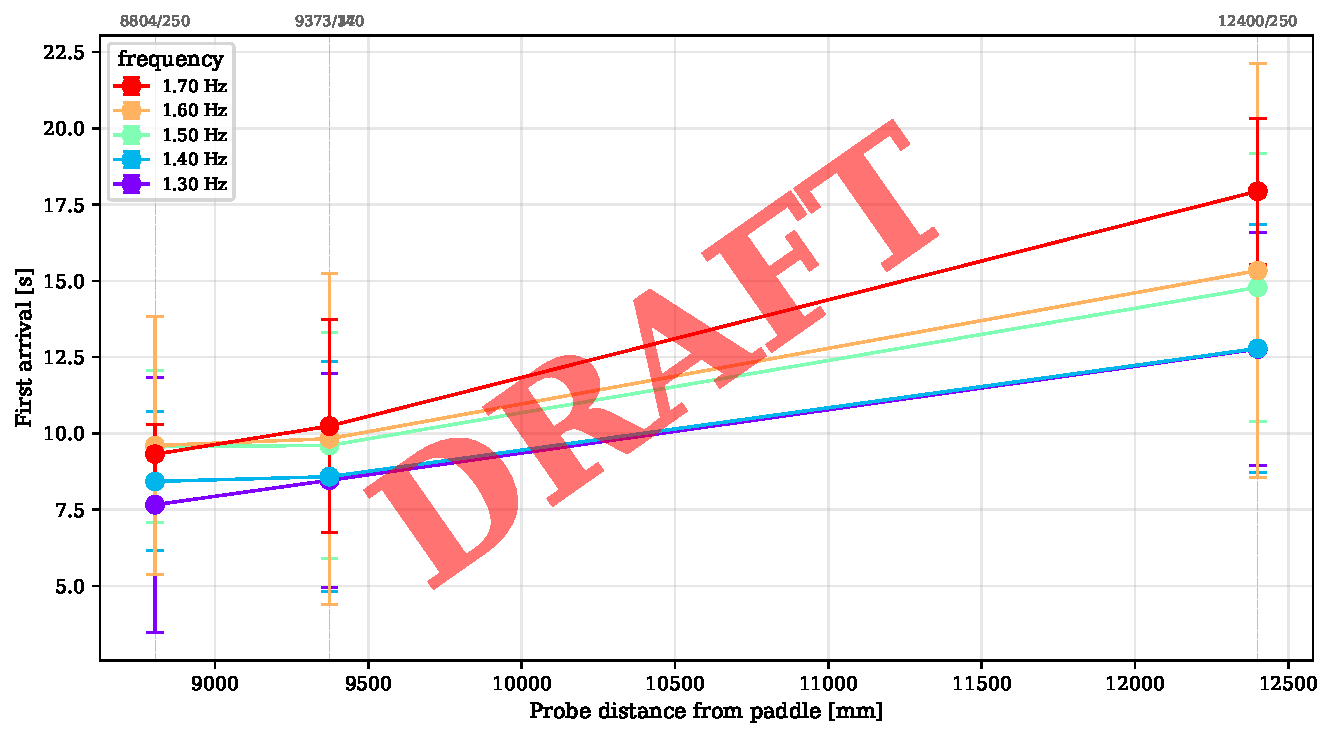
\includegraphics[width=0.9\linewidth]{FIGURES/ch04_first_arrival.pdf}
  \caption[First wave arrival time at each probe vs]{
    First wave arrival time at each probe vs.\ distance from the paddle, no-wind runs (173 runs). Detection: rolling 2.5\,s window exceeds 5.0$\times$ stillwater noise floor (9373/170: 0.90\,mm, 12400/250: 0.77\,mm, 9373/340: 0.61\,mm, 8804/250: 0.74\,mm). Arrivals $\leq$0.5\,s excluded as instrument transients. Error bars: half-range across parallel probes at the same longitudinal distance.
  }
  \label{fig:ch04_first_arrival}
\end{figure}
